
%%%%%%%%%%%%%%%%%%%%%%%%%%%%%%%%%%%%%%%%%%%%%%%%%%%%%%%%%%%%%%%%%%%%%%%%%%%%%%%%%%%%%%%
%%%%%%%%%%%%%%%%%%%%%%%%%%%%%%%%%%%%%%%%%%%%%%%%%%%%%%%%%%%%%%%%%%%%%%%%%%%%%%%%%%%%%%%
% 
% This top part of the document is called the 'preamble'.  Modify it with caution!
%
% The real document starts below where it says 'The main document starts here'.

\documentclass[12pt]{article}
\usepackage{hyperref}

\usepackage{amssymb,amsmath,amsthm}
\usepackage[top=1in, bottom=1in, left=1.25in, right=1.25in]{geometry}
\usepackage{fancyhdr}
\usepackage{enumerate}
\usepackage{listings}
\usepackage{graphicx}
\usepackage{float}
\usepackage{multicol}
% Comment the following line to use TeX's default font of Computer Modern.
\usepackage{times,txfonts}
\usepackage{mwe}
\usepackage{caption}
\usepackage{subcaption}

\usepackage{tikz}
\def\checkmark{\tikz\fill[scale=0.4](0,.35) -- (.25,0) -- (1,.7) -- (.25,.15) -- cycle;} 



\makeatletter
\renewcommand*\env@matrix[1][*\c@MaxMatrixCols c]{%
  \hskip -\arraycolsep
  \let\@ifnextchar\new@ifnextchar
  \array{#1}}
\makeatother

\newtheoremstyle{homework}% name of the style to be used
  {18pt}% measure of space to leave above the theorem. E.g.: 3pt
  {12pt}% measure of space to leave below the theorem. E.g.: 3pt
  {}% name of font to use in the body of the theorem
  {}% measure of space to indent
  {\bfseries}% name of head font
  {:}% punctuation between head and body
  {2ex}% space after theorem head; " " = normal interword space
  {}% Manually specify head
\theoremstyle{homework} 

% Set up an Exercise environment and a Solution label.
\newtheorem*{exercisecore}{\@currentlabel}
\newenvironment{exercise}[1]
{\def\@currentlabel{#1}\exercisecore}
{\endexercisecore}

\newcommand{\localhead}[1]{\par\smallskip\noindent\textbf{#1}\nobreak\\}%
\newcommand\solution{\localhead{Solution:}}

%%%%%%%%%%%%%%%%%%%%%%%%%%%%%%%%%%%%%%%%%%%%%%%%%%%%%%%%%%%%%%%%%%%%%%%%
%
% Stuff for getting the name/document date/title across the header
\makeatletter
\RequirePackage{fancyhdr}
\pagestyle{fancy}
\fancyfoot[C]{\ifnum \value{page} > 1\relax\thepage\fi}
\fancyhead[L]{\ifx\@doclabel\@empty\else\@doclabel\fi}
\fancyhead[C]{\ifx\@docdate\@empty\else\@docdate\fi}
\fancyhead[R]{\ifx\@docauthor\@empty\else\@docauthor\fi}
\headheight 15pt

\def\doclabel#1{\gdef\@doclabel{#1}}
\doclabel{Use {\tt\textbackslash doclabel\{MY LABEL\}}.}
\def\docdate#1{\gdef\@docdate{#1}}
\docdate{Use {\tt\textbackslash docdate\{MY DATE\}}.}
\def\docauthor#1{\gdef\@docauthor{#1}}
\docauthor{Use {\tt\textbackslash docauthor\{MY NAME\}}.}
\makeatother

% Shortcuts for blackboard bold number sets (reals, integers, etc.)
\newcommand{\Reals}{\ensuremath{\mathbb R}}
\newcommand{\Nats}{\ensuremath{\mathbb N}}
\newcommand{\Ints}{\ensuremath{\mathbb Z}}
\newcommand{\Rats}{\ensuremath{\mathbb Q}}
\newcommand{\Cplx}{\ensuremath{\mathbb C}}
%% Some equivalents that some people may prefer.
\let\RR\Reals
\let\NN\Nats
\let\II\Ints
\let\CC\Cplx

%\textbf{Code:}
%\begin{center}
%  \lstinputlisting{NewtonsMethodP5.m}
%\end{center}
%
%\textbf{Console:}
%\begin{center}
%  \lstinputlisting{P5C.txt}
%\end{center}
%\vspace{.15in}


%\begin{figure}[H]
%  \begin{center}
%    \caption{The one-norm unit ball}
%    \includegraphics[width=.76\textwidth]{1norm.png}
%  \end{center}
%\end{figure}




%%%%%%%%%%%%%%%%%%%%%%%%%%%%%%%%%%%%%%%%%%%%%%%%%%%%%%%%%%%%%%%%%%%%%%%%%%%%%%%%%%%%%%%
%%%%%%%%%%%%%%%%%%%%%%%%%%%%%%%%%%%%%%%%%%%%%%%%%%%%%%%%%%%%%%%%%%%%%%%%%%%%%%%%%%%%%%%
% 
% The main document start here.

% The following commands set up the material that appears in the header.
\doclabel{Math 615: Homework 8}
\docauthor{Stefano Fochesatto}
\docdate{\today}


\begin{document}


\begin{exercise}{Problem P34} Consider the heat equation $u_t = Du_{xx}$ for $D > 0$ constant, $x \in [0,1]$ and Dirichlet boundary conditions $u(t, 0) = 0$ and $u(t, 1) = 0$. Suppose we have initial condition $u(0, x) = \sin(5\pi x)$. 
  \begin{enumerate}
    \item[\textbf{a}] Confirm that, 
    \begin{equation*}
      u(t, x) = e^{-25\pi^2Dt}\sin(5\pi x)
    \end{equation*}
    is an exact solution. 
    \solution Note that the second derivative with respect to $x$ gives, 
    \begin{equation*}
      u_{xx} = -(5\pi)^2e^{-25\pi^2Dt}\sin(5\pi x).
    \end{equation*}
    The first derivative with respect to $t$ gives, 
    \begin{equation*}
      u_{t} = -25\pi^2De^{-25\pi^2Dt}\sin(5\pi x) =  D(-(5\pi)^2e^{-25\pi^2Dt}\sin(5\pi x)) = Du_{xx}.
    \end{equation*}
    And clearly this solution satisfies the Dirichlet conditions since $\sin(0) = \sin(5\pi) = 0$, as well as the initial condition since $e^{-25\pi^2D(0)} = e^0 = 1$. Therefore this is an exact solution to the problem. 
    \vspace*{.15in}


    \item[\textbf{b}] Implement the backward Euler method, as applied to MOL ODE system, to solve this heat equation problem. Specifically, use diffusivity $D = 1/20$ and final time $t_f = .1$. Note that you do not need to use Newton's method to solve the implicit equation, a linear system, but you should use sparse storage and a linear solver. 
    \solution\\
    \textbf{Code:}
    \begin{center}
      \lstinputlisting[basicstyle = \footnotesize]{r1.txt}
    \end{center}
    \vspace*{.15in}





    \item[\textbf{c}] Suppose we set $k = h$ for the 'refinement path'. What do you expect for the convergence $O(h^p)$? Then measure it by suing the exact solution from $\textbf{a)}$, at the final time, and the infinity norm $||\cdot||_{\infty}$ and $h = .02, .01, .005, .002, .001, .0005$. Make a log-log convergence plot of $h$ versus error. 
    \solution

      \begin{figure}[H]
        \begin{center}
          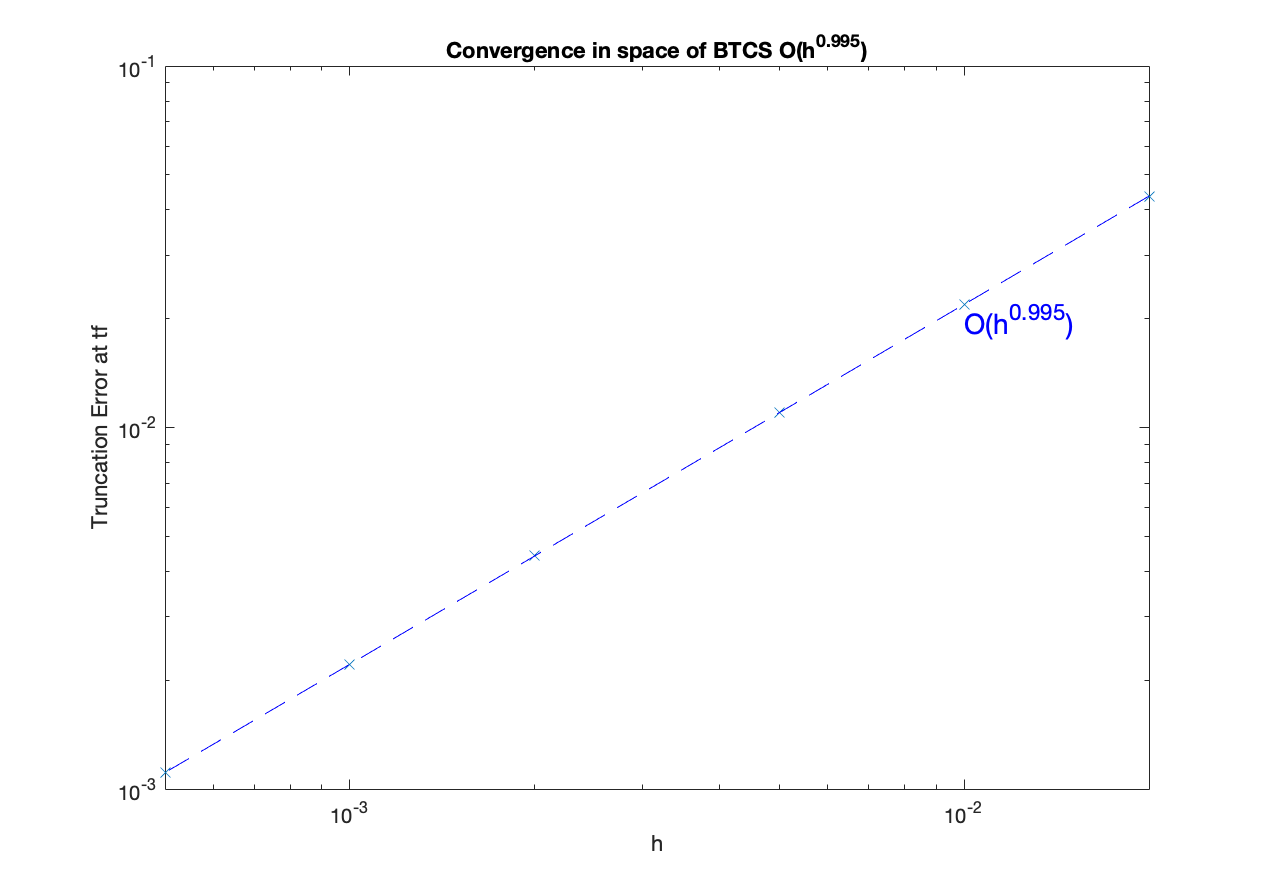
\includegraphics[width=.85\textwidth]{convergenceBTCS.png}
        \end{center}
      \end{figure}
    

    \textbf{Code:}
    \begin{center}
      \lstinputlisting[basicstyle = \footnotesize]{r2.txt}
    \end{center}
    \vspace*{.15in}



    \item[\textbf{d}] Repeat parts b and c but with the trapezoidal rule. Use 
    the same refinement path. Add the result to the same plot. 
    \solution The following is the code for trapezoid rule applied to the MOL ODE system as before,\\ 
    \textbf{Code:}
    \begin{center}
      \lstinputlisting[basicstyle = \footnotesize]{r3.txt}
    \end{center}

    \begin{figure}[H]
      \begin{center}
        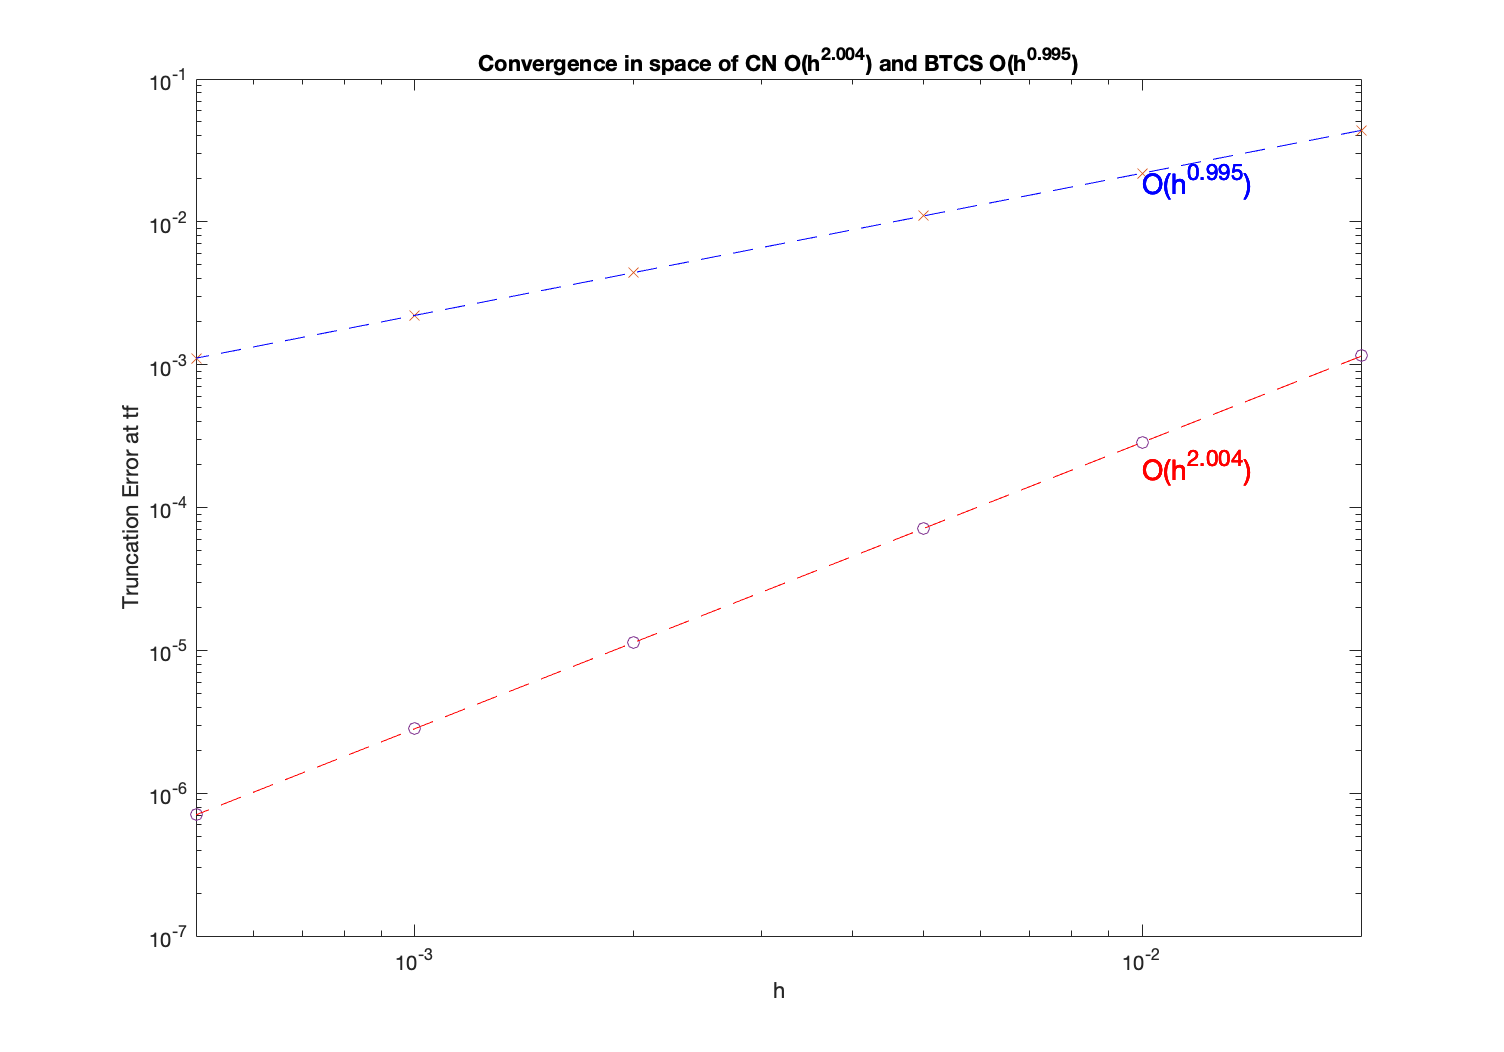
\includegraphics[width=.85\textwidth]{convergencFigCN.png}
      \end{center}
    \end{figure}

    \vspace*{.15in}





  \end{enumerate}
\end{exercise}
\vspace{.15in}





\begin{exercise}{Problem P35} Consider the following scheme, which applies centered differences to both sides of the heat equation $u_t = u_{xx}$:
  \begin{equation*}
    U_j^{n+2} = U_j^n + \frac{2k}{h^2}( U_{j-1}^{n+1}-2U_j^{n+1}+ U_{j+1}^{n+1})
  \end{equation*}
  \begin{enumerate}
    \item[\textbf{a}] Compute the truncation error to determine the order of accuracy of this method, in space and time. The answer will be in the form $\tau(t, x) = O(k^p + h^q)$; determine $p, q$.
    \solution The truncation error for the richardson scheme is based on the form, 
      \begin{equation*}
        \dfrac{U_j^{n+2} -  U_j^n}{2k} =\dfrac{U_{j-1}^{n+1}-2U_j^{n+1}+ U_{j+1}^{n+1}}{h^2}.
      \end{equation*}
      Note the following, 
      \begin{equation*}
        \tau(x, t+k) =   \dfrac{u(x, t+2k) -  u(x, t)}{2k} - \dfrac{u(x - h, t + k) -2u(x, t + k)+u(x + h, t + k)}{h^2}.
      \end{equation*}
      Let $u^{+k} = u(x , t + k)$. We will proceed by expanding all terms about $u^{+1}$ with Taylor's Theorem. Doing so we get that, 
      \begin{align*}
        \tau(x, t+k) = \dfrac{1}{2k} \biggl(&\bigl(u^{+k} - ku_{t}^{+k} + \frac{1}{2}k^2u_{tt}^{+k} - \frac{1}{6}k^3u_{ttt}^{+k} + \frac{1}{24}k^4u_{tttt}^{+k} + O(k^5)\bigr)\\ 
        &- \bigl(u^{+k} + ku_{t}^{+k} + \frac{1}{2}k^2u_{tt}^{+k} + \frac{1}{6}k^3u_{ttt}^{+k} + \frac{1}{24}k^4u_{tttt}^{+k} + O(k^5)\bigr)\biggr)\\
        -\frac{1}{h^2}\biggl(&\bigl(u^{+k} + hu_{x}^{+k} + \frac{1}{2}h^2u_{xx}^{+k} + \frac{1}{6}h^3u_{xxx}^{+k} + \frac{1}{24}h^4u_{xxxx}^{+k} + O(h^5)\bigr)\\
        &-2u^{+k}\\
        &+ \bigl(u^{+k} - hu_{x}^{+k} + \frac{1}{2}h^2u_{xx}^{+k} - \frac{1}{6}h^3u_{xxx}^{+k} + \frac{1}{24}h^4u_{xxxx}^{+k} + O(h^5)\bigr)
        \biggr)
      \end{align*}

      \begin{align*}
        \tau(x, t+k) = \dfrac{1}{2k} \biggl(&\bigl(- 2ku_{t}^{+k} - \frac{1}{3}k^3u_{ttt}^{+k} + O(k^6)\bigr)\biggr)\\
        -\frac{1}{h^2}\biggl(&\bigl(h^2u_{xx}^{+k} + \frac{1}{12}h^4u_{xxxx}^{+k} + O(h^6)\bigr)\biggr)
      \end{align*}
      \begin{align*}
        \tau(x, t+k) &= u_{t}^{+k} -  \frac{1}{6}k^2u_{ttt}^{+k} + O(k^5) - u_{xx}^{+k} - \frac{1}{12}h^2u_{xxxx}^{+k} + O(h^4)\\
        &= - \frac{1}{6}k^2u_{ttt}^{+k} - \frac{1}{12}h^2u_{xxxx}^{+k} + O(h^4) + O(k^5)
      \end{align*}
      Therefore we have shown that the truncation error for this scheme is order $O(k^2 + h^2)$.
  

      \vspace*{.15in}




      \item[\textbf{b}] Derive the method by applying the midpoint ODE method, to the MOL ODE system (9.10). 
      Also, find the region of absolute stability of the midpoint method; it is in the textbook. Is 
      the method likely to generate reasonable results? Why or why not?
      \solution Recall the midpoint ODE method, 
      \begin{equation*}
        \dfrac{U^{n + 1} - U^{n - 1}}{2k} = f(U^n).
      \end{equation*}
      Also recall the MOL ODE system from 9.10, 
      \begin{equation*}
        U'_i(t) = \frac{1}{h^2}\left(U_{i - 1}(t) - 2U_i(t) + U_{i + 1}(t)\right)\qquad \text{i = 1,2, \dots $m$}
      \end{equation*}
      Which can be written in matrix vector form, where $A$ is the typical tridiagonal matrix,
      \begin{equation*}
        U'(t) = AU(t).
      \end{equation*}
      Applying Midpoint ODE method where $f(U^n) = AU(t)$, a matrix multiplication we get a new system, 
      \begin{equation*}
        \dfrac{U^{n + 1} - U^{n - 1}}{2k} = AU^n.
      \end{equation*}
      Considering the $i^{th}$ row of this system we get the desired richardson scheme, 
      \begin{equation*}
        \dfrac{U_i^{n + 1} - U_i^{n - 1}}{2k} = \frac{1}{h^2}\left(U_{i - 1}^n - 2U_i^n + U_{i + 1}.^n\right)
      \end{equation*}

      To find the region of absolute stability of the midpoint method, we apply the scheme to the test equation $u' = \lambda u$. Doing so we get, 
      \begin{equation*}
        \dfrac{U^{n + 2} - U^{n}}{2k} = \lambda U^{n+1}
      \end{equation*}
      Solving for the latest step we get, 
      \begin{equation*}
        U^{n + 2} = U^{n} + 2k\lambda U^{n+1} = U^{n} + 2zU^{n+1}.
      \end{equation*}
      Solving this linear recurrence relation we substitute $U^{n} = \zeta^n$ ($n$ is a power on the the the RHS), with $\zeta \neq 0$ and we get, 
      \begin{align*}
        \zeta^{n+2} &=  \zeta^{n} + 2z\zeta^{n+1},\\
        \zeta^{n+2} - 2z\zeta^{n+1} - \zeta^{n}&= 0,\\
        \zeta^{2} - 2z\zeta^{1} - 1 &= 0.
      \end{align*}
      So we have our \emph{stability polynomial}, 
      \begin{equation*}
        \pi(\zeta;z) = \zeta^2 - 2z\zeta - 1
      \end{equation*}
      With roots $\zeta_{1, 2} = z \pm \sqrt{z^2 + 1}$. From our text we know that the region of absolute stability is given by all $z$ such that $|\zeta_i| \leq 1$, with a strict inequality whenever $\zeta_i$ is a repeated root. 
  \end{enumerate}
\end{exercise}


\begin{exercise}{Problem P36} Consider the Jacobi iteration for the linear system $Au = b$
  arising from a centered FD approximation fo the boundary value problem $u''(x) = f(x)$. 
  Show that this iteration can be interpreted as forward Euler time-stepping applied to a heat equation
  MOL system (9.10) with time step $k = \frac{1}{2}h^2$. 
  \solution Recall the forward Euler scheme and the MOL system described in 9.10. Note that $f_i = f(x_i)$,
  \begin{equation*}
    \dfrac{U^{n + 1} - U^{n}}{k} = f(U^n).
  \end{equation*}
  \begin{equation*}
    U'_i(t) = \frac{1}{h^2}\left(U_{i - 1}(t) - 2U_i(t) + U_{i + 1}(t)\right) + f_i\qquad \text{i = 1,2, \dots $m$} 
  \end{equation*}
  Just like before written in matrix vector form, where $A$ is the typical tridiagonal matrix and $f$ is the source described in $u_t(t, x) = u_{xx}(t, x) - f(x)$,
  \begin{equation*}
    U'(t) = AU(t) - f.
  \end{equation*}
  Applying forward Euler ODE method where $f(U^n) = AU(t) + f$, we get a new system, 
  \begin{equation*}
    \dfrac{U^{n + 1} - U^{n}}{k} = AU^n - f.
  \end{equation*}
  We recall that $k = \frac{1}{2}h^2$, so by substitution we get, 
  \begin{equation*}
    \dfrac{2U^{n + 1}}{h^2} - \frac{2U^{n}}{h^2} = AU^n + f.
  \end{equation*}  Adding the $\frac{2U^{n}}{h^2}$ term we remove the diagonal entries of $A$, so
  if $A = D - L - U$ we get $A - D = -(L + U)$ and therefore by substitution we get the desired Jacobi iteration,
  \begin{align*}
    \dfrac{2U^{n + 1}}{h^2} &= -(L + U)U^n - f,\\
    -\dfrac{2}{h^2}U^{n + 1} &= f + (L + U)U^n,\\
    DU^{n + 1} &= f + (L + U)U^n.
  \end{align*}


\end{exercise}


\end{document}











 




